\documentclass[crop,tikz,dvipsnames]{standalone}
\usepackage{xcolor}
\usepackage{amsfonts}
\usepackage{amsthm}
\usepackage{amsmath}
\usetikzlibrary{positioning}
\begin{document}
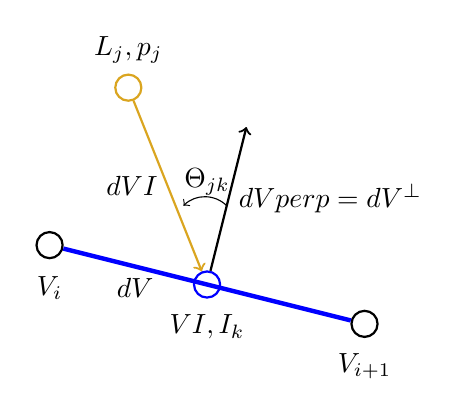
\begin{tikzpicture}
  \node[draw, thick, circle, Goldenrod, label={$L_{j}, p_{j}$}] (L) at (1,3) {};
  \node[draw, thick, circle, label={[yshift=-10mm]$V_{i}$}] (V1)  at (0,1) {};
  \node[draw, thick, circle, label={[yshift=-10mm]$V_{i+1}$}] (V2) at (4,0) {};
  \node[draw, thick, circle, blue, label={[yshift=-10mm]$VI, I_{k}$}] (VI) at (2,0.5) {};
  \draw[-, ultra thick,blue] (V1) -- (V2) node[near start,below,black] {$dV$};
  \draw[->, thick] (VI) -- ++(0.5,2) node[midway,right] {$dVperp = dV^{\perp}$};
  \draw[->, thick,Goldenrod] (L) -- (VI) node[midway,left,black] {$dVI$};
  \draw[->, bend angle=45, bend right] (2.25,1.5) to (1.7,1.5);
  \node[] at (2,1.8) {$\Theta_{jk}$};
\end{tikzpicture}
\end{document}
